\documentclass{article}
\usepackage{graphicx}
\begin{document}
\newcommand{\exercice}[1]{\section{#1}}
\exercice{Utilisation d'int\'egrales d\'efinies}
Calculez les int\'egrales suivantes~:
\begin{enumerate}
\item $\displaystyle \int_{x=0}^\infty x^3\exp^{(-2x^2)}dx$
\item $\displaystyle \int_{\theta=0}^\infty \frac{\exp^{(-5\theta)}-\exp^{(-\pi\theta)}}{\theta} d\theta$
\item $\displaystyle \int_{r=0}^\infty r^n\exp^{(-1.902r)}dr$
\end{enumerate}
Calculez les int\'egrales suivantes en fonction de $\alpha$~:
\begin{enumerate}
\item $\displaystyle \int_{y=0}^\infty y^7\exp^{(-\alpha y^2)}dy$
\item $\displaystyle \int_{\phi=0}^\infty \phi^{5}\exp^{(-\alpha\phi^2)}d\phi$
\item $\displaystyle \int_{r=0}^\infty r^n\exp^{(-\alpha r)}dr$
\item $\displaystyle \int_{r=0}^\infty\int_{\theta=0}^\infty\int_{\phi=0}^\infty \phi^{5}\exp^{(-\alpha\phi^2)}r^n\exp^{(-\beta r)} \frac{\exp^{(-5\theta)}-\exp^{(-\pi\theta)}}{\theta} drd\theta d\phi$
\end{enumerate}
Donn\'ees~:
\begin{itemize}
\item $\displaystyle \int_{t=0}^\infty t^{2n+1}\exp^{-at^2}dt = \frac{n!}{2a^{n+1}}$
\item $\displaystyle \int_{t=0}^\infty \frac{\exp^{-at} - \exp^{-bt}}{t}dt = \ln\frac{b}{a}$
\item $\displaystyle \int_{t=0}^\infty t^n\exp^{-at}dt = \frac{n!}{a^{n+1}}$
\end{itemize}
\exercice{Coordonn\'ees sph\'eriques}
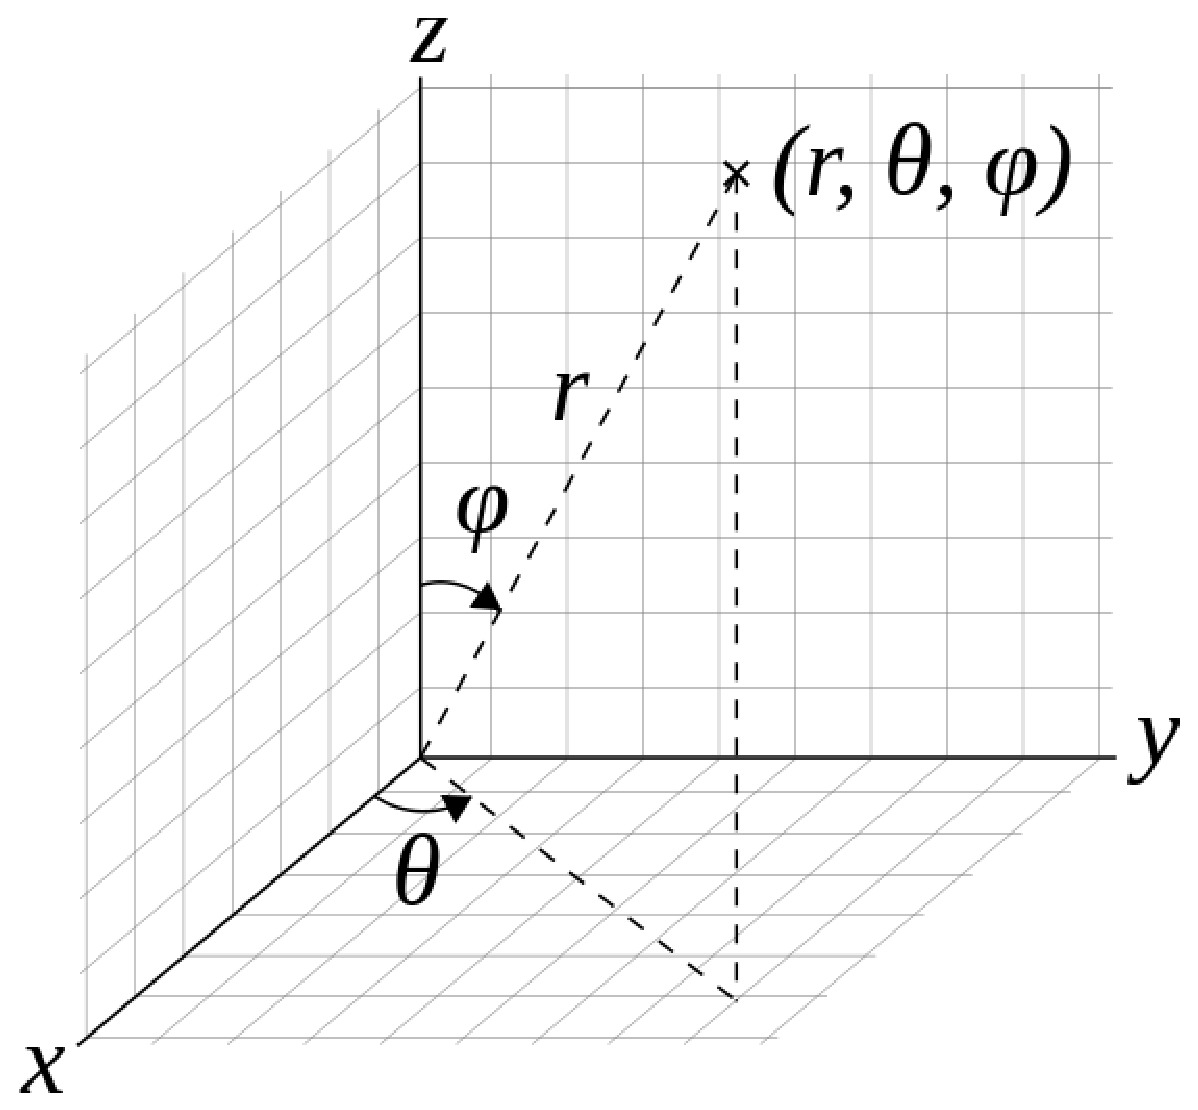
\includegraphics[height=10cm]{spheriques.eps}\\
Le passage des coordonn\'ees cart\'esiennes $(x,y,z)$ aux coordonn\'ees sph\'eriques $(r,\theta,\phi)$
se fait selon les formules suivantes~:
\begin{itemize}
\item $x=r\sin\theta\cos\phi$
\item $y=r\sin\theta\sin\phi$
\item $z=r\cos\theta$
\item $r=\sqrt{x^2+y^2+z^2}$
\item $\phi = \arctan\frac{y}{x}$
\item $\theta = \arccos\frac{z}{r}$
\end{itemize}
Soient les points suivants en coordonn\'ees cart\'esiennes, calculez leur coordonn\'ees sph\'eriques~:
\begin{itemize}
\item $M_x(1,0,0)$, $M_y(0,1,0)$, $M_z(0,0,1)$
\item $P_{x,y}(1,1,0)$ $P_{x,z}(1,0,1)$ $P_{y,z}(0,1,1)$ et $P_{x,y,z}(1,1,1)$
\item $Q_{x,y}(1,-1,0)$ $Q_{x,z}(1,0,-1)$ $Q_{y,z}(0,-1,1)$ et $Q_{x,y,z}(-1,-1,-1)$
\end{itemize}
Lesquels de ces points sont-ils sur la m\^eme sph\`ere?

%% Int\'egrez sur tout l'espace les fonctions suivantes en coordonn\'ees sph\'eriques en fonction des param\`etres $\alpha$
%% et $\beta$ si n\'ecessaire~:
%% \begin{enumerate}
%% \item $f(r,\theta,\phi) = 1$
%% \item $g(r,\theta,\phi) = r$
%% \item $h(r,\theta,\phi) = r\phi$
%% \item $i(r,\theta,\phi) = \frac{r^2}{\sin\theta}$
%% \item $j(r,\theta,\phi) = r^\alpha\exp(-\beta\phi)(\sin\theta)^{-1}$
%% \end{enumerate}
\exercice{Soit un objet sph\'erique dont la densit\'e massique $\rho$ varie en
fonction de $r$}
En coordonn\'ees sph\'eriques $(r,\theta,\phi)$ l'\'el\'ement de volume sur lequel on int\`egre
s'\'ecrit $dV=r^2\sin(\theta)drd\theta d\phi$.

Calculez sa masse si :
\begin{enumerate}
\item $\rho(r)=1$;
\item $\rho(r)=r^{2}$; $r<=3cm$;
\item $\rho(r)=5-r$;
\item $\rho(r)=5-r^{2}$;
\item $\rho(r)=\exp^{(-\zeta r)}$ sachant que $\int_{0}^{\infty}x^{n}\exp^{-ax}dx=\frac{n!}{a^{n+1}}$;
\item $\rho(r)=\exp^{(-\alpha r^{2})}$ sachant que $\int_{0}^{\infty}x^{2}\exp^{-ax^{2}}dx=\frac{\sqrt{\pi}}{4\sqrt{a}}$
;
\end{enumerate}
$\rho(r)$ ne peut pas \^etre n\'egative.

\end{document}
